\documentclass[11pt,answers]{exam}

\usepackage{etex}
\usepackage{amssymb,amsmath,multicol} %<-- InWorksheetExam1 i also have fancyhdr,

\usepackage{hyperref}


\usepackage[metapost]{mfpic}
\usepackage[pdftex]{graphicx}

\usepackage{pst-plot}
\usepackage{pgfplots}
\pgfplotsset{compat=1.9}

\usepackage{tikz}
\usepackage{tkz-2d}
\usepackage{tkz-base}
\usetikzlibrary{calc}

\usepackage[inline]{enumitem}
\usepackage{refcount}%<-- non in WorksheetExam1



%\renewcommand{\headrulewidth}{0pt}

\newcommand{\vasymptote}[2][]{
    \draw [densely dashed,#1] ({rel axis cs:0,0} -| {axis cs:#2,0}) -- ({rel axis cs:0,1} -| {axis cs:#2,0});
}

\makeatletter
\newcommand{\inlineitem}[1][]{%
\ifnum\enit@type=\tw@
    {\descriptionlabel{#1}}
  \hspace{\labelsep}%
\else
  \ifnum\enit@type=\z@
       \refstepcounter{\@listctr}\fi
    \quad\@itemlabel\hspace{\labelsep}%
\fi}
\makeatother


\addpoints
%\printanswers
\noprintanswers

\opengraphsfile{Exam2aaa_Spring_15}

\begin{document}
\extrawidth{-0.3in}
\pagestyle{headandfoot}

\setlength{\hoffset}{-.25in}

\extraheadheight{-.4in}
\runningheadrule
\firstpageheader{\bfseries {MATH1-UC 1171}}{ \bfseries {Exam 2 }}{\bfseries {5/12/2015}} 



\firstpagefooter{\bfseries{}}{}{} 


\runningheader{\bfseries {}}%
              {\bfseries {}}%
              {Page \thepage\ 
							of \numpages 
							}
\runningfooter{} %%&&CHANGED
                {}
                {Points earned: \hbox to 0.5in{\hrulefill}
                 out of  \pointsonpage{\thepage} points}
                 
						

\vspace*{0.2cm}
\hbox to \textwidth { \scshape {Name:} \enspace\hrulefill}
\vspace{0.2in}

\begin{itemize}
	\item This exam contains \numpages\ pages, including this cover page, the unit circle page and the blank last page which you can tear out and use as scrap paper. Enter
your name on the top of this page, and put your initials
on the top of every page. Please note that I will not grade anything that you write on the last (blank) page.

%\item Please read the instructions for each individual problem carefully. Try not to overthink a problem and read between the lines! Take your time to solve each problem, and don't rush to finish!
%\item Write legibly and clearly label your answers. If I cannot read your solution to a problem, the problem will receive a score of zero.
\item Calculators may not be used in this exam. You may use your note-card with fomulas/examples. 

\item Please write your name on your note-card and include it in your exam. If you do not have a note-card, please write {\textit {no note-card}} on this page.
\item Turn off all phones and computers, and remove all headphones.
\item Cheating is a violation of the SPS policy on academic integrity. The SPS statement on academic integrity and
plagiarism is available at \url{http://tinyurl.com/ko3f79s}. The academic integrity disciplinary procedures outlined on the
website will be strictly enforced.

\end{itemize}

For the problems where you are required to show your work, the following rules apply:\\

\begin{minipage}[t]{3.7in}
\vspace{0pt}
\begin{itemize}

\item \textbf{Include explanations in complete sentences or step-by-step calculations}. If you draw a graph, you must label the axes, include tick marks and include units both on the horizontal and vertical axis. If you are asked to explain in practical terms, then your explanation cannot contain math symbols or formulas.
\item \textbf{Use the methods described in this course} as part of your explanations: for example, you cannot use derivatives to find the peaks and valley of a function.

\item \textbf{Organize your work}, neatly and legibly in
the space provided. Work that is disorganized and difficult to read will not receive full credit.  

\item \textbf{A correct answer, unsupported by calculations, explanation,
or algebraic work will receive no credit}; an incorrect answer supported
by  calculations and explanations may receive
partial credit.


\item \textbf{If you need more space}, use the back of the pages; clearly indicate when you have done this.
\end{itemize}

Do not write in the table to the right.
\end{minipage}
\hfill
\begin{minipage}[t]{2.3in}
\vspace{0pt}
%\cellwidth{3em}
\gradetablestretch{2}
\vqword{Pages}
\addpoints % required here by exam.cls, even though questions haven't started yet.	
\combinedgradetable[v][pages]  % Use [pages] to have grading table by page instead of question

\end{minipage}
\newpage

%\bigskip

%\begin{center}
%\gradetable[v][pages]
%\end{center}

%\newpage

\pointpoints{point}{points}

\begin{questions}


\addpoints
%\qformat{Question \thequestion\dotfill
%         {(\pointsofquestion{\arabic{question}} \points)}}

%\bonusqformat{Bonus Question \thequestion\dotfill
%         {(\bonuspointsofquestion{\arabic{question}} \points)}}        
        
%%%%%%%%%%%%%%%%
\question  For each equation below, find the exact solution(s). Show your work step by step and write your answer(s) on each answer line.

\begin{parts}
\part[2] (Explanations are required.) $\displaystyle \log(x)+\log(x+3)=1$
\fillwithdottedlines{1.8in}

Exact solution(s):\dotfill

\part[2] (Explanations are required.) $\displaystyle \log \left(10^{2x}\right)=\log\left (10^{3x}\right)+1$
\fillwithdottedlines{1.8in}

Exact solution(s):\dotfill

\part[2] (Explanations are required.) $\displaystyle 2\left (3^{4x}\right )=5^x$
\fillwithdottedlines{1.8in}

Exact solution(s):\dotfill

\end{parts}

\question[2] (Explanations are required.) Find the $y$-coordinate of $P$, using the fact that P lies on the unit circle in the second quadrant, and that its $x$-coordinate is $\displaystyle -\frac{5}{13}$.

\fillwithdottedlines{0.8in}

The $y$-coordinate of $P$ is:\dotfill

\bonusquestion[1] Is there a number whose natural log is $-1000000$?
\begin{oneparchoices}
\choice Yes \choice No
\end{oneparchoices}

\newpage
 \question The graph of one period of a trigonometric function  is shown below:

\begin{mfpic}[35][50]{0}{5.25}{-1.15}{1.5}
\point[3pt]{(1.5708,0), (2.3562,1), (3.1415,0), (3.927,-1), (4.7124,0)}
\axes
\tlabel[cc](5.25,-0.25){$x$}
\tlabel[cc](0.25,1.5){$y$}
\xmarks{1.5708, 2.3562, 3.1415, 3.927, 4.7124}
\ymarks{-1,1}
\tlpointsep{4pt}
\axislabels {x}{{$\frac{\pi}{2}$} 1.5708, {$\frac{3\pi}{4}$} 2.3562, {$\pi$} 3.1415, {$\frac{5\pi}{4}$} 3.927, {$\frac{3\pi}{2}$} 4.7124}
\axislabels {y}{{$-1$} -1, {$1$} 1}
\function{1.5708, 4.7124, 0.1}{sin(2*x - 3.1415)}
\end{mfpic}

\begin{parts}
\part[1] The amplitude is: \dotfill
\part[1] The period is: \dotfill
\part[3] (Explanations are required.) Write  an equation that represents the curve in the form
$\displaystyle y = a \sin k(x - b)$. Explain how you find $a$, $k$ and $b$, and write your equation in the space provided below.
\fillwithdottedlines{0.8in}

The equation is $y=$\dotfill
\part[2] (Explanations are required.) Write  an equation that represents the curve in the form
$\displaystyle y = a \cos k(x - b)$. Write your equation in the space provided below.
\fillwithdottedlines{0.8in}

The equation is $y=$\dotfill

\end{parts}


\question Each time your heart beats, your blood pressure first increases and then decreases as the heart rests between beats. The maximum and minimum blood pressures are called the systolic and diastolic pressures, respectively. Your blood pressure reading is written as systolic/diastolic. A reading of 120/80 is considered normal.

A certain person's blood pressure is modeled by the function
$\displaystyle p(t) = 125 + 25 \sin(150\pi t)$
where $p(t)$ is the pressure in mmHg (millimeters of mercury), at time $t$ measured in minutes.

\begin{parts}

\part[3] (Explanations are required.) Find the blood pressure reading.
\fillwithdottedlines{1in}

systolic/diastolic =    \hbox to 0.5in{\dotfill}  /   \hbox to 0.5in{\dotfill}  

\part[1] How does this compare to normal blood pressure?
\begin{oneparchoices}
\choice This reading is lower than normal.
\choice This reading is normal.    
\choice This reading is higher than normal.
\end{oneparchoices}
\end{parts}

\newpage
\bonusquestion[1] What is the period of the function $\displaystyle y=\cos\left (\frac{x}{60}\right )$? \dotfill
\question[2] Write the domain of $\displaystyle y=\sin^{-1}(x)$ in interval form. \dotfill
\question[2] Write the range of $\displaystyle y=\sin^{-1}(x)$ in interval form. \dotfill
\question[1] Which of the following is {\emph{not}} true?
\begin{enumerate*}[label=\textcolor{red}{\bf (\alph*)}]
\item $\displaystyle \sin^{-1}\left (\sin \left(\frac{\pi}{4}\right )\right )=\frac{\pi}{4}$
\inlineitem $\displaystyle \sin^{-1}\left (\sin \left(\frac{9\pi}{4}\right )\right )=\frac{9\pi}{4}$
\end{enumerate*}
\begin{oneparchoices}
\choice (a) is not true
\choice (b) is not true   
\end{oneparchoices}
\question Find the exact value of each expression. If an expression is undefined, write {\sc {undefined}} on the answer line.
\begin{parts}
\part[1] $\displaystyle \sin^{-1}\left(\sin\left(\frac{2\pi}{3}\right )\right)$ \dotfill
\part[1] $\displaystyle \sin\left(\sin^{-1}\left(2\pi\right )\right)$ \dotfill
\part[1] $\displaystyle \cos^{-1}\left(\cos\left(\frac{17\pi}{6}\right )\right)$ \dotfill
\end{parts}

\question[4] (Explanations are required.) Graph one cycle of the function $\displaystyle y = \cos(3x - 2\pi) + 4$. Find the coordinates of all peaks and valleys  in the cycle you have drawn, and label them on your graph

\fillwithdottedlines{4cm}


\begin{tikzpicture}

    \draw[gray!50, thin, step=0.5] (-7,-4) grid (7,4);
    %\draw[very thick,->] (-7,0) -- (7.2,0) node[right] {$x$};
    %\draw[very thick,->] (0,-4) -- (0,4.2) node[above] {$y$};

\end{tikzpicture}

\newpage
\question[1] Is the following statement true or false? A rational function must have at least one vertical asymptotes.
\begin{oneparchoices}
\choice True \choice False
\end{oneparchoices}
\question[1] Is the following statement true or false? If a rational function has a horizontal asymptote, then the graph of the function may cross the horizontal asymptote.
\begin{oneparchoices}
\choice True
\choice False
\end{oneparchoices}
\question[1] Is the following statement true or false? Every rational function must have at least one $x$-intercept.
\begin{oneparchoices}
\choice True
\choice False
\end{oneparchoices}
\question[1] When $x\to \infty$ then:

\begin{oneparchoices}
\choice  $\displaystyle \frac{2x(x+3)}{(x^2+2)(x-5)}\to 2$
\choice  $\displaystyle \frac{2x(x+3)}{(x^2+2)(x-5)}\to 0$
\choice  $\displaystyle \frac{2x(x+3)}{(x^2+2)(x-5)}\to \infty$
\end{oneparchoices}

\question  The graph of the rational function $\displaystyle y=\frac{f(x)}{g(x)}$ is shown below.

\begin{minipage}[t]{0.49\linewidth}
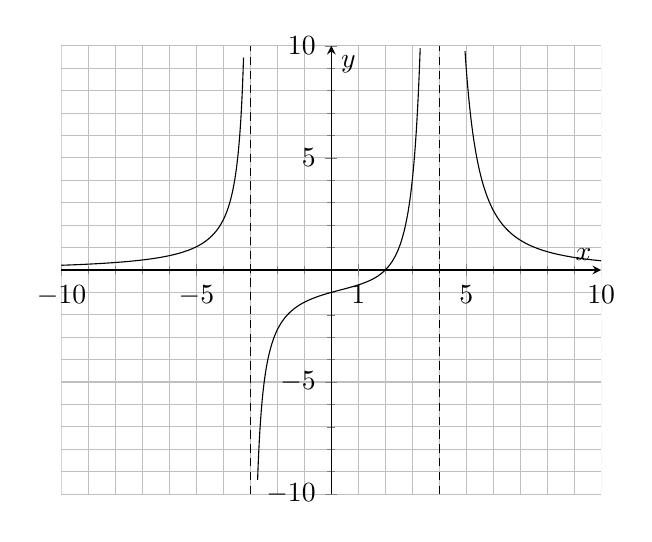
\begin{tikzpicture}
    \begin{axis}[
        restrict y to domain=-10:10,
        samples=1000,
        minor tick num=4,
        xmin = -10, xmax = 10,
        ymin = -10, ymax = 10,
        unbounded coords=jump,
        axis x line=middle,
        axis y line=middle, grid=both,
        extra x ticks={1},
        %extra x tick style={grid=major,
        %tick label style={
        %rotate=90,anchor=east}},
        extra x tick labels={1},
        xlabel=$x$,ylabel=$y$]

      \addplot[mark=none, domain=-10:10] {(-48+24*x)/(x^3-5*x^2-8*x+48)};
      \vasymptote {-3}
      \vasymptote {4}
    \end{axis}
  \end{tikzpicture}
  \end{minipage}
\hfill \vrule \hfill
\begin{minipage}[b]{0.5\linewidth}

\begin{parts}
\part[2] Write the equations of the vertical asymptotes. \dotfill


\part[2] Write the equations of the horizontal asymptote. \dotfill


\part[2] Which of the following best represents the denominator $g(x)$ of the rational function? 

\begin{enumerate}
\item $\displaystyle (x+3)^2(x-4)^2$
\item $\displaystyle (x+3)(x-4)^2$
\item $\displaystyle (x+3)^2(x-4)$
\item $\displaystyle (x+3)(x-4)$
\item None of the above
\end{enumerate}

\end{parts}
\end{minipage}

%\fillwithdottedlines{0.5in}

\question A population is modeled by the function 
$\displaystyle P(t) = 
\frac{120t}{t + 20}$, where  $t$ represents the number of years after 1803. 
\begin{parts}
\part[1] Find the horizontal asymptote of the graph of 
$y = P(t)$.

The horizontal asymptote is: \dotfill 

\bonuspart[1] Which of the following options best describes the meaning of the horizontal asymptote in practical terms?  Circle the {\underline{one}} best answer.
\begin{enumerate}[label= \fbox{\bf  \alph*}]
\item  The model predicts that the population  will never exceed 6.
\item  The model predicts that the population  will never be below 20.    
\item  The model predicts that the population  will never exceed 120.
\item The model predicts that the population  will never be below 120.
\item  The model predicts that the population  will never exceed 20.
\end{enumerate}
\end{parts}
\newpage
\question[2] (Explanations are required.) A population grows exponentially and triples in size every twenty years. The initial population is one million. What is the doubling time of this population? Write your answer in exact form (not in decimal form) and simplify as much as possible.
\fillwithdottedlines{0.7in}

The doubling time is:\dotfill

\question[2] (Explanations are required.) How much money will you have at the end of four years if you deposit \$10000 a year (at the end of each year) into a bank account paying 0.6\% interest? Write your answer in exact form (not in decimal form) and simplify as much as possible.
\fillwithdottedlines{0.7in}

Money in the account at the end of four years:\dotfill

\question Let $\displaystyle g(x)=-2^{-x}$.
\begin{parts}


\part[2] List the function transformations of $ \displaystyle f(x)=2^x$ that result in $g(x)$.
\fillwithdottedlines{0.7in}

\part[3] Graph $g(x)$. [Include units, label the $y$-coordinate of the $y$ intercept and draw the horizontal asymptote as a dashed line.]

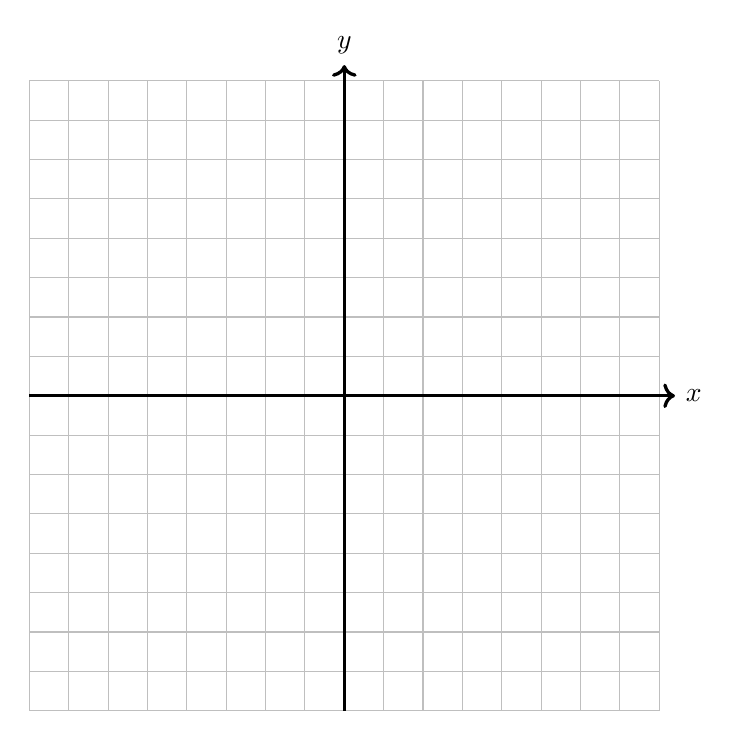
\begin{tikzpicture}

    \draw[gray!50, thin, step=0.5] (-4,-4) grid (4,4);
    \draw[very thick,->] (-4,0) -- (4.2,0) node[right] {$x$};
    \draw[very thick,->] (0,-4) -- (0,4.2) node[above] {$y$};

\end{tikzpicture}

\part[2] Write the range of $g(x)$ in interval form. \hbox to 0.9in{\dotfill}

\part[1] Write the equation of the horizontal asymptote of $g(x)$. \hbox to 0.9in{\dotfill}
\end{parts}

\question[2]  Expand $\displaystyle \log_5 \left(\left(\frac{z}{25}\right )^3\right )$ using the properties of logarithms and simplify. Assume when necessary that $z$ represents a positive real number. Simplify your answer as much as possible.

\fillwithdottedlines{0.7in}
$\displaystyle \log_5 \left(\left(\frac{z}{25}\right )^3\right )=$\dotfill 

\question (Explanations are required.) Evaluate each expression and simplify your answer as much as possible.
\begin{parts}
\part[1] $\displaystyle \log_8 0.5$
\fillwithdottedlines{0.5in}
\part[1] $\displaystyle \ln\left (\frac{1}{e}\right )$
\fillwithdottedlines{0.5in}
\part[1] $\displaystyle \log\left (100000\right )$
\fillwithdottedlines{0.5in}
\part[1] $\displaystyle \log_6 9+\log_6 4$
\fillwithdottedlines{0.5in}
\end{parts}
\question[2] (Explanations are required.) Write the equation of the function of the form $\displaystyle f(x)=\log_a x$ which passes through the point $(10,1)$.
\fillwithdottedlines{0.7in}
$\displaystyle f(x)=$\dotfill 

\question Find the exact value of each expression:
\begin{parts}
\part[1] $\displaystyle \sin \left (\frac{\pi}{2}\right)$ \dotfill 
\part[1] $\displaystyle \sin \left (-\frac{\pi}{2}\right)$ \dotfill 
\part[1] $\displaystyle \sin \left (\frac{5\pi}{2}\right)$ \dotfill
\part[1] $\displaystyle \sin \left (-\frac{5\pi}{2}\right)$ \dotfill 
\end{parts}

\question[2] (Explanations are required.) Find the present value of \$10,000 if interest is paid at a rate of 0.8\% per year, compounded semiannually, for 2 years. Write your answer in exact form (not in decimal form) and simplify as much as possible.
\fillwithdottedlines{0.7in}

Present value:\dotfill
\question[2] (Explanations are required.) The graph of one period of a trigonometric function is shown below. Write an equation for the function.

\smallskip

\begin{minipage}[b]{0.40\textwidth}%[4cm][c]{6cm}
\begin{tikzpicture}[yscale=2]
\tkzInit[xmin=0,xmax=2,ymin=-1.25,ymax=1.25]
\tkzY[gradsize=\scriptstyle]
\tkzX %[trig=2]
\draw[color=blue,samples at={0,0.1,...,2.1
}] plot (\x,{cos(3.14*\x r)})%
node[above] {$ $};
%\draw[color=black,samples at={-6.28,-6.24,...,6.28}] plot (\x,{cos(\x r)})%
node[above] {$ $};
\end{tikzpicture}
\end{minipage}
\begin{minipage}[b]{0.60\textwidth}%[6.5cm][c]{6cm}
\fillwithdottedlines{2in}

Equation:\dotfill
\end{minipage}
\medskip
\bonusquestion[2] (Explanations are required.) Graph the function $\displaystyle P(x)=\frac{120x}{x+20}$. Label all asymptotes and intercepts, and explain how you sketch the graph. 
\fillwithdottedlines{1.2in}


\begin{tikzpicture}
\draw[gray!50, thin, step=0.5] (-7,-3) grid (7,3);
    \end{tikzpicture}

\end{questions}
\newpage


\thispagestyle{empty}

    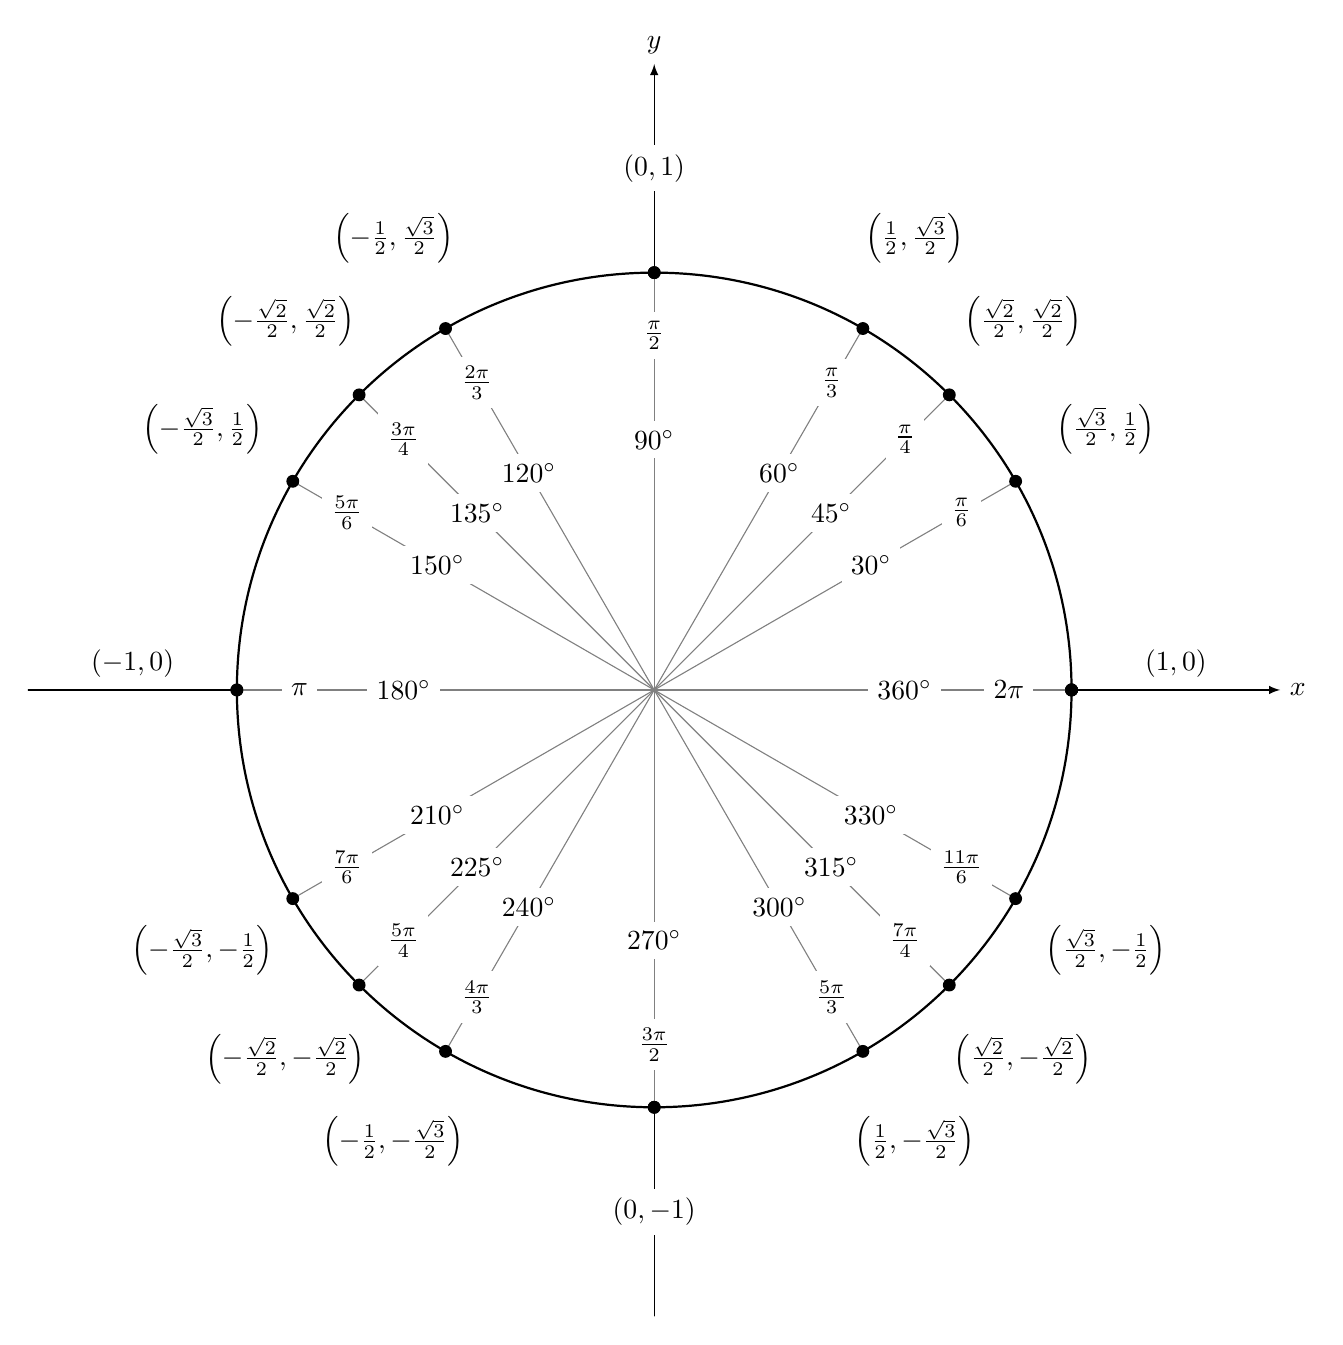
\begin{tikzpicture}[scale=5.3,cap=round,>=latex]
        % draw the coordinates
        \draw[->] (-1.5cm,0cm) -- (1.5cm,0cm) node[right,fill=white] {$x$};
        \draw[->] (0cm,-1.5cm) -- (0cm,1.5cm) node[above,fill=white] {$y$};

        % draw the unit circle
        \draw[thick] (0cm,0cm) circle(1cm);

        \foreach \x in {0,30,...,360} {
                % lines from center to point
                \draw[gray] (0cm,0cm) -- (\x:1cm);
                % dots at each point
                \filldraw[black] (\x:1cm) circle(0.4pt);
                % draw each angle in degrees
                \draw (\x:0.6cm) node[fill=white] {$\x^\circ$};
        }
        
        \foreach \x in {0,45,...,360} {
                % lines from center to point
                \draw[gray] (0cm,0cm) -- (\x:1cm);
                % dots at each point
                \filldraw[black] (\x:1cm) circle(0.4pt);
                % draw each angle in degrees
                \draw (\x:0.6cm) node[fill=white] {$\x^\circ$};
        }
        % draw each angle in radians
        \foreach \x/\xtext in {
            30/\frac{\pi}{6},
            45/\frac{\pi}{4},
            60/\frac{\pi}{3},
            90/\frac{\pi}{2},
            120/\frac{2\pi}{3},
            135/\frac{3\pi}{4},
            150/\frac{5\pi}{6},
            180/\pi,
            210/\frac{7\pi}{6},
            225/\frac{5\pi}{4},
            240/\frac{4\pi}{3},
            270/\frac{3\pi}{2},
            300/\frac{5\pi}{3},
            315/\frac{7\pi}{4},
            330/\frac{11\pi}{6},
            360/2\pi}
                \draw (\x:0.85cm) node[fill=white] {$\xtext$};

        \foreach \x/\xtext/\y in {
            % the coordinates for the first quadrant
            30/\frac{\sqrt{3}}{2}/\frac{1}{2},
            45/\frac{\sqrt{2}}{2}/\frac{\sqrt{2}}{2},
            60/\frac{1}{2}/\frac{\sqrt{3}}{2},
            % the coordinates for the second quadrant
            150/-\frac{\sqrt{3}}{2}/\frac{1}{2},
            135/-\frac{\sqrt{2}}{2}/\frac{\sqrt{2}}{2},
            120/-\frac{1}{2}/\frac{\sqrt{3}}{2},
            % the coordinates for the third quadrant
            210/-\frac{\sqrt{3}}{2}/-\frac{1}{2},
            225/-\frac{\sqrt{2}}{2}/-\frac{\sqrt{2}}{2},
            240/-\frac{1}{2}/-\frac{\sqrt{3}}{2},
            % the coordinates for the fourth quadrant
            330/\frac{\sqrt{3}}{2}/-\frac{1}{2},
            315/\frac{\sqrt{2}}{2}/-\frac{\sqrt{2}}{2},
            300/\frac{1}{2}/-\frac{\sqrt{3}}{2}}
                \draw (\x:1.25cm) node[fill=white] {$\left(\xtext,\y\right)$};

        % draw the horizontal and vertical coordinates
        % the placement is better this way
        \draw (-1.25cm,0cm) node[above=1pt] {$(-1,0)$}
              (1.25cm,0cm)  node[above=1pt] {$(1,0)$}
              (0cm,-1.25cm) node[fill=white] {$(0,-1)$}
              (0cm,1.25cm)  node[fill=white] {$(0,1)$};
    \end{tikzpicture}




\newpage


\thispagestyle{empty}


\setlength\fboxrule{2pt}\setlength\fboxsep{2mm}
\fbox{This page is intentionally left blank.} You may use it as scrap paper for your calculations.
\end{document}                 